\section{Zusammenfassung und Diskussion}
	Im Experiment wurde die mittlere Lebensdauer von Myonen mit Hilfe einer Koinzidenzmessung untersucht. Zur Abschätzung wurde das Maximum-Likelihood-Verfahren eingesetzt, wobei drei verschiedene Verteilungen zugrunde gelegt wurden: ein exponentielles Zerfallsgesetz, eine Poisson- und eine Normalverteilung. Tabelle \ref{tab:results} fasst die Ergebnisse für die Kanäle 20 bis 175 zusammen.
	\begin{table}[ht]
		\centering
		\begin{tabular}{c|c}
		Verteilung & mittlere Lebensdauer $\tau /\unit{\mu s}$\\
		\hline
		Exponentielles Zerfallsgesetz	&	$3,52 \pm 0,03$\\
		Poissonverteilung				&	$2,24 \pm 0,03$\\
		Normalverteilung 				&	$2,23 \pm 0,01$
		\end{tabular}
		\caption{Schätzwerte für die mittlere Lebensdauer der Myonen.}
		\label{tab:results}
	\end{table}
	Man beobachtet, dass die Ergebnisse für die Poisson- und die Normalverteilung sehr gut zum Literaturwert (\ref{eq:lit}) passen. Das exponentielle Zerfallsgesetz kommt nur mit einer anderen Kanalkonstellation an dieses Ergebnis heran, weshalb diese Methode nicht die optimale Wahl zur Schätzung dieses Parameters ist. Die Genauigkeit des Ergebnisses wird vor allem durch zufällige Koinzidenzen begrenzt. Der $\mu^-$-Einfang sollte dafür keine große Rolle spielen, da die dabei entstehenden Zerfallsprodukte kein Stoppsignal $2 \cdot \bar{3}$ oder $\bar{2} \cdot 3$ auslösen. Es sei denn, sie treten gemeinsam mit einer zufälligen Koinzidenz auf. Man könnte die Messung verbessern, indem man die Detektoren besser von der natürlich auftretenden Strahlung abschirmt. Zur exakteren Bestimmung der Lebensdauer könnte man Myonen durch Pion-Erzeugung an einem Teilchenbeschleuniger beobachten und vermessen.
	

\newpage
\section{Anhang}
In diesem Abschnitt befindet sich das handschriftlich erstellte Messprotokoll mitsamt der uns gegebenen Aufgabenstellung.\\
\begin{figure}[htbp]
    \subfigure[Aufgabenstellung]{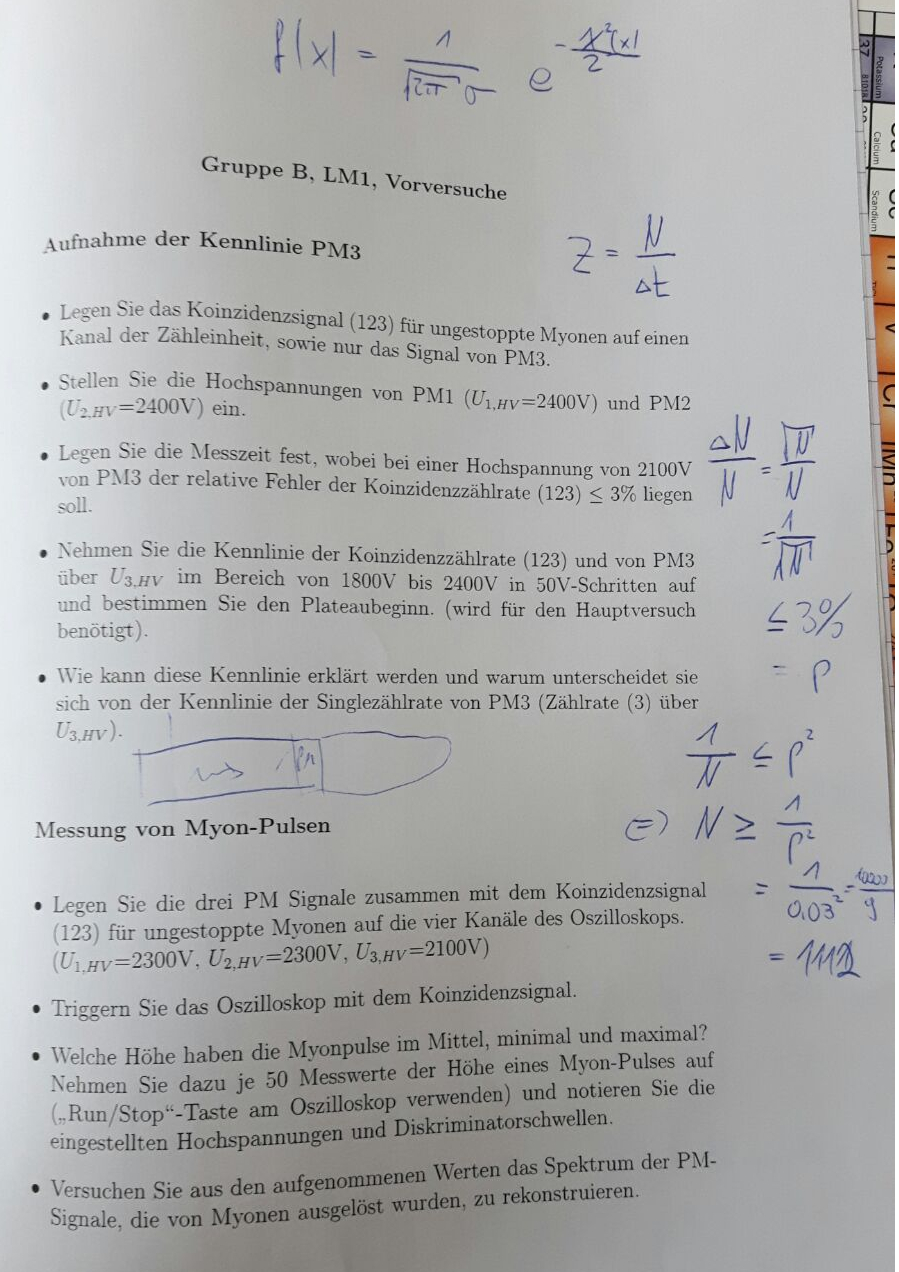
\includegraphics[scale=0.6]{pic/aufgabe.jpg}}
    \subfigure[S1, handschrftl. MP]{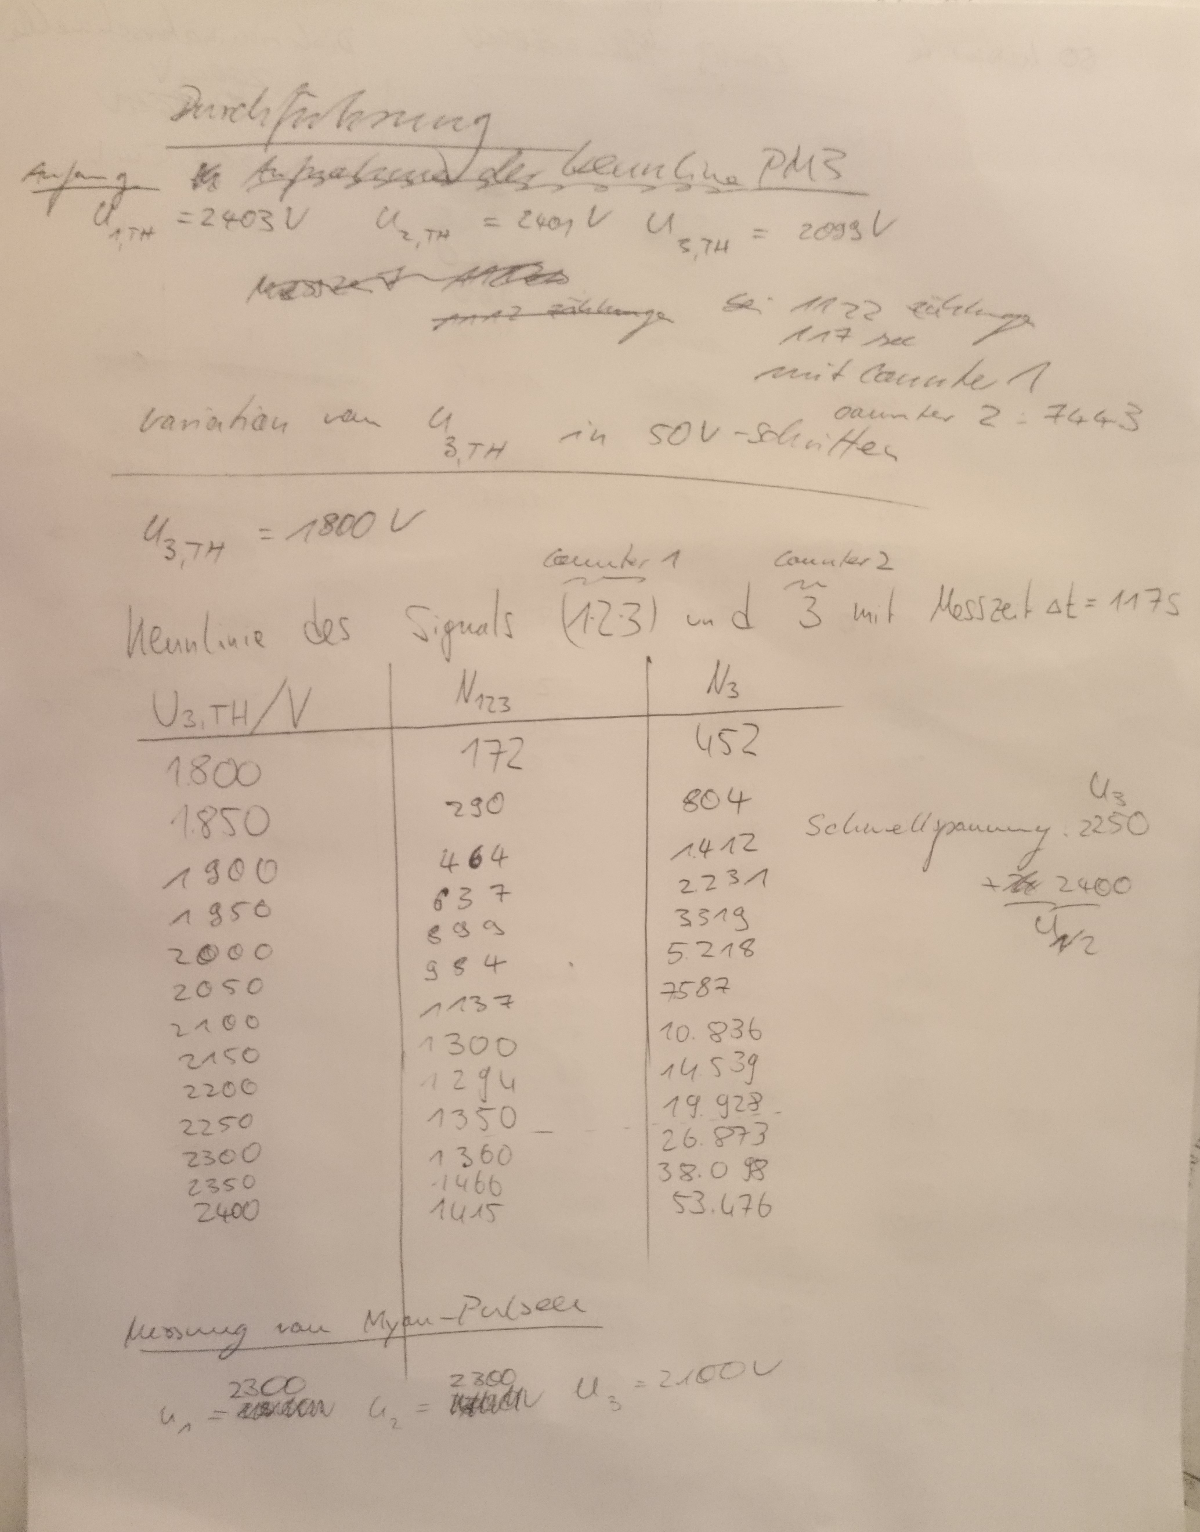
\includegraphics[scale=0.12]{pic/mess1.png}}
    \centering \subfigure[S2, handschiftl. MP]{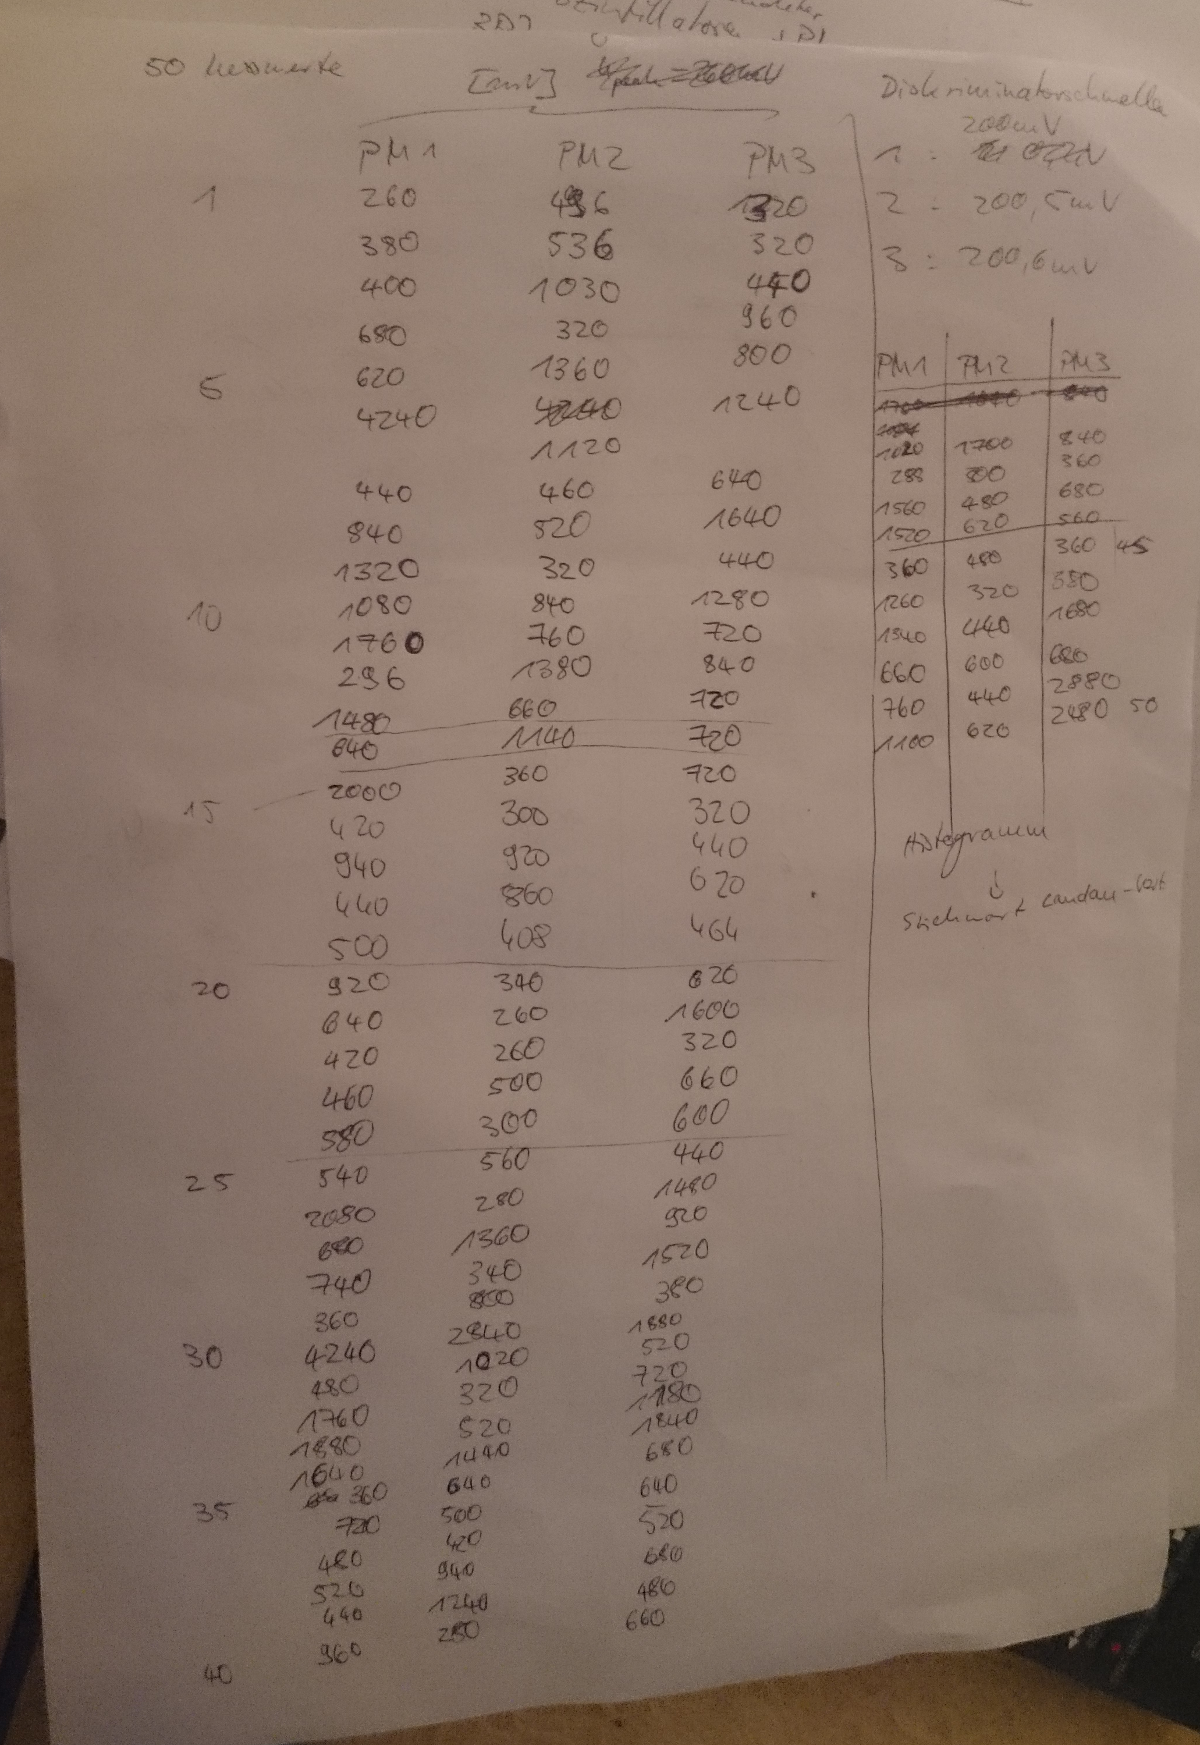
\includegraphics[scale=0.10]{pic/mess2.png}}
    \caption{Messprotokollseiten}
\end{figure}